%% =====================================================================
%%  APA 7th Edition — Student Paper Template (LaTeX)
%%
%%  Created by:  Parisa Rostami
%%  Source:      https://github.com/ParisaRostaami/APA7-LaTeX-Template
%%  Version:     1.0 (October 2026)
%%  License:     CC BY-NC 4.0  https://creativecommons.org/licenses/by-nc/4.0/
%%               The license covers this template. The paper you write
%%               with it is entirely your own.
%%
%%  Built on the `apa7` class by Daniel A. Weiss (CTAN) and the
%%  `biblatex-apa` style by Philip Kime.
%%
%%  HOW TO USE
%%   1. Fill in the title-page fields in the "TITLE PAGE" block below.
%%   2. Write your paper between \maketitle and \printbibliography.
%%   3. Put your sources in references.bib and cite them with
%%        \parencite{key}  ->  (Author, 2020)
%%        \textcite{key}   ->  Author (2020)
%%   4. Compile with:  pdfLaTeX -> Biber -> pdfLaTeX -> pdfLaTeX
%%      (Overleaf does this automatically.)
%%
%%  Lines starting with % are comments and do not appear in the PDF.
%% =====================================================================

% `stu`          = student paper (no running head; course/instructor/date on title page)
% `floatsintext` = tables and figures appear in the text, not at the end
% `12pt`         = APA-compliant size for Times New Roman
\documentclass[stu,12pt,floatsintext]{apa7}

% ---------- Language, font, references --------------------------------
\usepackage[american]{babel}
\usepackage[T1]{fontenc}
\usepackage{newtxtext,newtxmath}   % Times New Roman look (APA-approved font)
\usepackage{csquotes}              % required by biblatex-apa
\usepackage[style=apa,sortcites=true,sorting=nyt,backend=biber]{biblatex}
\DeclareLanguageMapping{american}{american-apa}
\addbibresource{references.bib}

% ---------- Useful extras (optional) ----------------------------------
\usepackage{graphicx}   % \includegraphics for figures
\usepackage{booktabs}   % clean table rules (\toprule, \midrule, \bottomrule)
\usepackage{amsmath}    % equations
\hypersetup{hidelinks}   % apa7 already loads hyperref; this removes colored link boxes
% Note: the apa7 class already sets 1-inch margins, double spacing,
% 0.5-inch paragraph indents, and page numbers in the top-right corner.

% =====================================================================
%  TITLE PAGE  — edit everything in this block
% =====================================================================
\title{Title of Your Paper in Title Case: Subtitle if Needed}

% Student name(s). Multiple authors:  \authorsnames{First Author, Second Author}
\authorsnames{Student Full Name}

% Department and university
\authorsaffiliations{{School of Computing, Wichita State University}}

\course{CS 000: Course Name}
\professor{Prof. Instructor Name}
\duedate{Month Day, Year}

% Abstract and keywords are NOT required for student papers unless your
% instructor asks for them. To omit, delete (or comment out) both lines.
\abstract{Write a single paragraph of 150--250 words summarizing the
purpose, method, key findings, and implications of your work. The abstract
is not indented.}
\keywords{keyword one, keyword two, keyword three}

% =====================================================================
\begin{document}
\maketitle
% The paper title is repeated automatically at the top of the first page
% of text, so do NOT add an "Introduction" heading here (APA rule).

Start your introduction here. Every paragraph is indented 0.5 inches and the
whole paper is double-spaced. You do not need to do anything to get this
formatting; the template handles it.

When citing a source in parentheses, use \verb|\parencite|: deep learning
models have transformed computer vision \parencite{lecun2015deep}. When the
author is part of the sentence, use \verb|\textcite|: \textcite{lecun2015deep}
reviewed the field. For two authors, APA uses ``\&'' inside parentheses and
``and'' in the sentence: \parencite{sutton2018reinforcement} versus
\textcite{sutton2018reinforcement}. For three or more authors, APA shortens to
``et al.'' from the first citation: \parencite{vaswani2017attention}.
Multiple sources in one parenthesis are ordered alphabetically:
\parencite{vaswani2017attention,lecun2015deep}. For a direct quotation, add a
page number: \parencite[p.~437]{lecun2015deep}.

\section{Level 1 Heading: Centered, Bold, Title Case}

Text begins as a new, indented paragraph below the heading.

\subsection{Level 2 Heading: Flush Left, Bold, Title Case}

Text begins as a new paragraph.

\subsubsection{Level 3 Heading: Flush Left, Bold Italic, Title Case}

Text begins as a new paragraph.

\paragraph{Level 4 Heading Indented, Bold, Title Case, Ending With a Period}
Text begins on the same line and continues as a regular paragraph.

\subparagraph{Level 5 Heading Indented, Bold Italic, Title Case, Ending With a
Period} Text begins on the same line and continues as a regular paragraph.

\section{Tables and Figures}

Refer to every table and figure in the text, for example
Table~\ref{tab:results} and Figure~\ref{fig:example}. APA places the bold
number above the italic title; the template does this for you.

Equations are numbered on the right and can be referenced like tables, as in
Equation~\ref{eq:f1}:
\begin{equation}
  F_1 = 2 \cdot \frac{\text{Precision} \cdot \text{Recall}}{\text{Precision} + \text{Recall}}
  \label{eq:f1}
\end{equation}

\begin{table}[htbp]
  \caption{Classification Performance of Each Model on the Test Set}
  \label{tab:results}
  {\centering
  \begin{tabular}{lccc}
    \toprule
    Model & Accuracy & Precision & Recall \\
    \midrule
    Logistic regression & .82 & .80 & .79 \\
    Random forest       & .87 & .86 & .85 \\
    CNN                 & .91 & .90 & .92 \\
    \bottomrule
  \end{tabular}\par}
  \vspace{0.5\baselineskip}
  \figurenote{Values are proportions. APA omits the leading zero for values that cannot exceed 1.}
\end{table}

\begin{figure}[htbp]
  \caption{Training and Validation Accuracy Across 20 Epochs}
  \label{fig:example}
  {\centering
  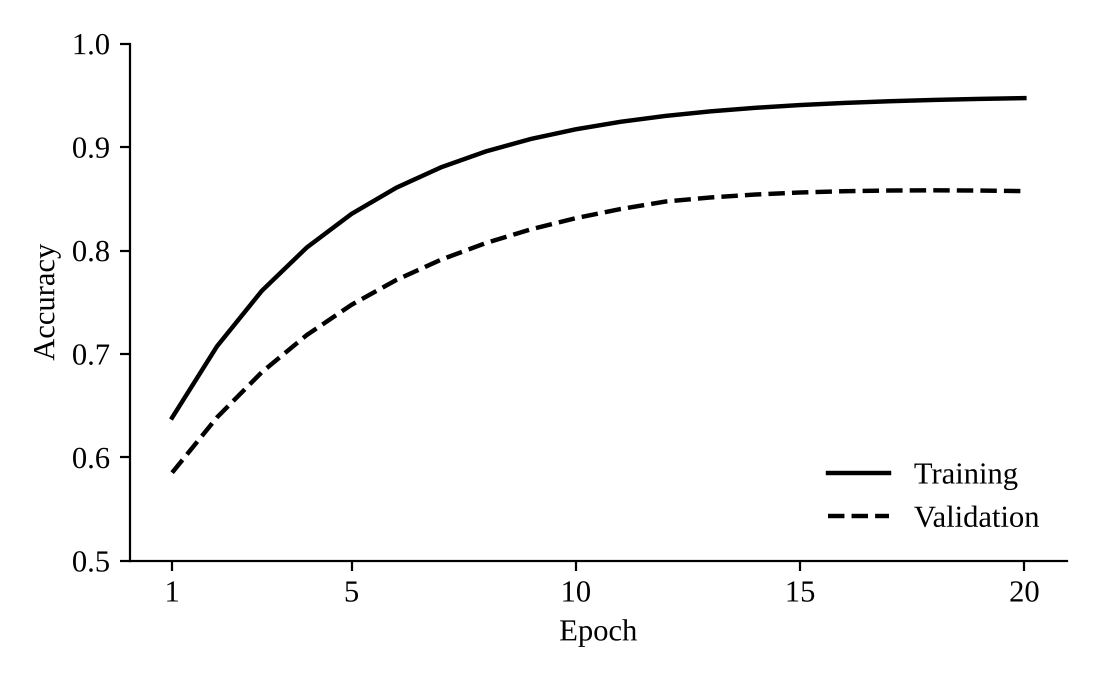
\includegraphics[width=0.75\linewidth]{figures/sample-figure.png}\par}
  % Put your image files in the "figures" folder and change the file name above.
  \figurenote{Replace this figure with your own. Use the note to explain
  abbreviations or to credit the source of an adapted figure.}
\end{figure}

\section{Conclusion}

Summarize your main points here.

% ---------------------------------------------------------------------
%  REFERENCES — generated automatically from references.bib.
%  Only sources you actually cite will appear.
% ---------------------------------------------------------------------
\printbibliography

% ---------------------------------------------------------------------
%  APPENDIX (optional). Delete this block if you do not need it.
% ---------------------------------------------------------------------
\appendix
\section{Supplementary Material}

Appendices come after the references. Each one starts on a new page.

\end{document}
